\subsection{Prime-Time Ratio} \label{subsec:primetime}

The daily diurnal nature of Internet traffic demand requires that ISP providers 
design networks capable of handling load at the times when heaviest usage is 
observed. Such heavy demand is usually observed during prime time hours in the 
evening, when many subscribers heavily consume real-time entertainment traffic
(video) (seen as primarily responsible for high usage during these hours). The FCC defines 
\textbf{Prime-Time} as the local time from 7:00 PM to 11:00 PM.
\cite{fcc2014measuring-broadband}. To measure the concentration of network usage
during prime-time, we use Sandvine's definition of the \textbf{Prime-Time 
ratio}: the ratio of the average traffic demand during prime-time hours to the average 
traffic demand in non-prime-time hours.\cite{sandvine20141h, sandvine20142h}.

We measure the prime-time ratio of the \control{} and \treatment{} group
for each contiguous four hour period in our datasets to find the evening hours with
the largest prime-time ratio. We observed that in our dataset,
the prime time ratio consistently peaks at 8:00 PM -- 12:00 AM for both
datasets.

\begin{figure}[t]
\begin{minipage}{1\linewidth}
\centering
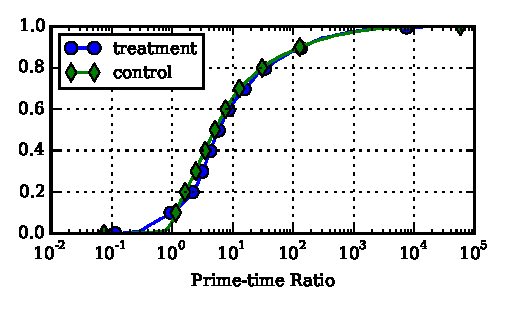
\includegraphics[width=1\linewidth]{figures/prime-time-ratio-per-device-cdf-MEAN.pdf}
\caption{Prime-Time Ratio\label{fig:cdf-prime-time-ratio}}
\end{minipage}
\end{figure}

\begin{table}[t]
\begin{tabular}{| cc | c |c | }\hline
  &                    & Weekday         & Weekends \\\hline
\multirow{2}{*}{\begin{tabular}[c]{@{}l@{}}Hourly Traffic in\\ Prime-Time\end{tabular}}              & treatment          & 233.12          & 246.93   \\
& control            & 225.40          & 238.15   \\\hline
\multirow{2}{*}{\textbf{\begin{tabular}[c]{@{}l@{}}Hourly Traffic in\\ Non-Prime-Time\end{tabular}}} & \textbf{treatment} & \textbf{124.18} & 49.38    \\
& \textbf{control}   & \textbf{45.08}  & 47.63   \\\hline
\end{tabular}
\caption{Hourly Traffic Demand during in prime-time hours (MB)\label{prime-time-demand}}
\end{table}

%\begin{subfigure}[]{.32\linewidth}
%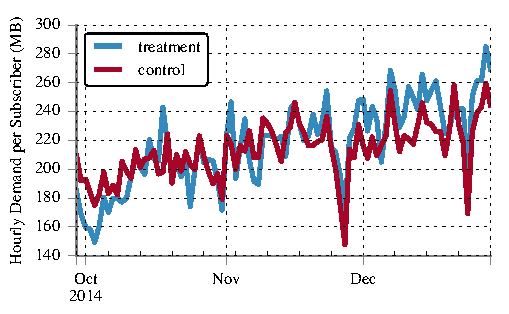
\includegraphics[width=1\linewidth]{figures/primetime_usage_per_day_per_subs.pdf}
%\caption{\label{fig:pt}}
%\end{subfigure}

%\begin{subfigure}[b]{.32\linewidth}
%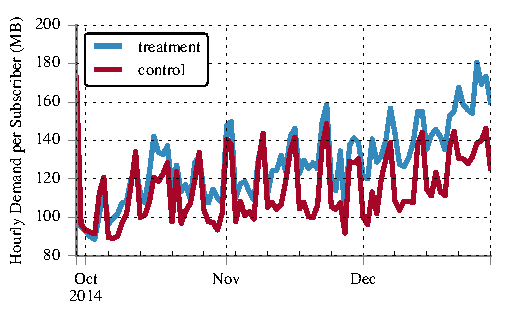
\includegraphics[width=1\linewidth]{figures/nonprimetime_usage_per_day_per_subs.pdf}
%\caption{\label{fig:non-pt}}
%\end{subfigure}


We observed that the hourly downlink traffic per 1000 subscribers between 8:00 PM -- 12:00 AM is 
209.5 GB for \treatment{}, and 205.1 GB for \control{}. However, during an average hour
outside of prime time, the traffic per 1000 subscribers is 122.3 GB for the higher tier
and 108.5 GB for the lower tier. This difference in demand during hours outside of the
daily prime-time is also apparant from the weekly usage patterns in Figure~\ref{fig:traffic-demand-timeseries}.
 
We calculate and plot the prime-time ratio per day for the \treatment{} and
\control{} groups in figure~\ref{fig:cdf-prime-time-ratio}. A comparison shows 
that the \treatment{} group's prime time ratio is unexpectedly 10\% lower than the 
\control{} group. This confirms our initial observation 
[\autoref{subsec:behavior}]
that the usage during peak evening hours is similar across both groups, but the
usage in off peak hours is higher in the \treatment{} group.


%Latency and performance 
%are adversely affected during prime-time, causing bottlenecks at home, the last 
%mile, in
%transit, or at the content server. For example, the Sandvine Global
%Internet Phenomena Report \footnote{The Sandvine Reports ~\cite{sandvine20141h,
%sandvine20142h}are released bi-annually and
%contain a detailed analysis of aggregate Internet usage. They are also referred
%to in the FCC reports~\cite{fcc2015progress-report, fcc2014measuring-broadband,
%fcc2014progress-report}} showed that devices in the same household selected  
%Netflix's own CDN (OpenConnect) during off-peak hours, and third party CDNs 
%(with differing
%performance) during prime-time. This may happen because Netflix OpenConnect is
%over-utilized during prime time~\cite{sandvine20141h}.